\begin{center}
	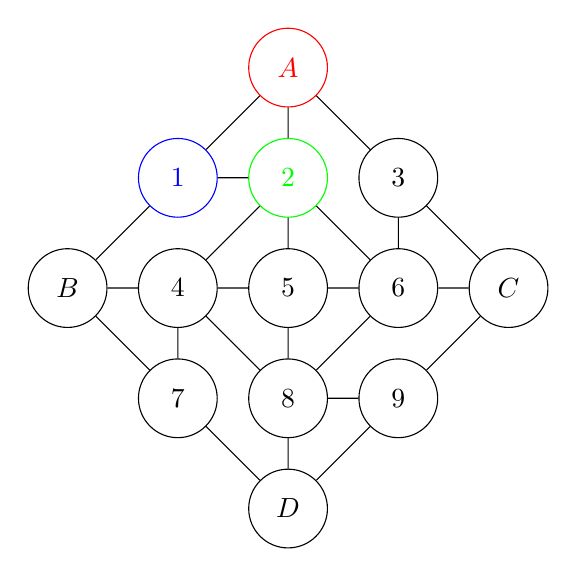
\begin{tikzpicture}[scale=1.4]
		\tikzset{nd/.style={circle, draw=black, minimum width=1cm}};

		\node[nd, red] (a) at (2, 4) {$A$};
		\node[nd, blue] (1) at (1, 3) {$1$};
		\node[nd, green] (2) at (2, 3) {$2$};
		\node[nd] (3) at (3, 3) {$3$};
		\node[nd] (b) at (0, 2) {$B$};
		\node[nd] (4) at (1, 2) {$4$};
		\node[nd] (5) at (2, 2) {$5$};
		\node[nd] (6) at (3, 2) {$6$};
		\node[nd] (c) at (4, 2) {$C$};
		\node[nd] (7) at (1, 1) {$7$};
		\node[nd] (8) at (2, 1) {$8$};
		\node[nd] (9) at (3, 1) {$9$};
		\node[nd] (d) at (2, 0) {$D$};

		\draw (a) to (1);
		\draw (a) to (2);
		\draw (a) to (3);

		\draw (1) to (2);
		\draw (1) to (b);

		\draw (2) to (4);
		\draw (2) to (5);
		\draw (2) to (6);

		\draw (3) to (6);
		\draw (3) to (c);

		\draw (b) to (4);
		\draw (b) to (7);

		\draw (4) to (5);
		\draw (4) to (7);
		\draw (4) to (8);

		\draw (5) to (8);
		\draw (5) to (6);

		\draw (6) to (c);
		\draw (6) to (8);

		\draw (c) to (9);

		\draw (7) to (d);
		
		\draw (8) to (d);
		\draw (8) to (9);

		\draw (9) to (d);
	\end{tikzpicture}
\end{center}
